% !TeX root = ./00.ppgcc-2020.tex

\chapter{Proposta e metodologia}\label{cha:proposta}

% \begin{resumocap}

  Este Capítulo apresenta a proposta deste trabalho e a metodologia elegida para
  atingir os objetivos.

% \end{resumocap}

In this work, we investigate an appropriate architecture for performing \nd at
the edge, as a means of allowing small IoT devices to filter and detect undesirable
network behavior.
Our approach is based on the \arch architecture \cite{Cassales2019a} and \nd
techniques provide by the \minas algorithm \cite{Faria2016minas}.
Named \mfog, our distributed algorithm explores load balancing to enable low
profile devices at the edge of the internet to also work on the classification
and detection of unwanted traffic.

In this work, we propose and assess \mfog, a distributed data stream
novelty detection system based on the algorithm \minas for securing \iot networks.
\mfog implements a distributed version of \minas according to the \arch
architecture proposed in a previous work \cite{Cassales2019a}, to execute in the
edge where small devices and constrained resources may be prevalent.

However, given the distributed nature and the typical use of small computing
devices in IoT scenarios, new challenges arise:

\begin{enumerate}[label=(\emph{\roman*})]
  \item the classification phase of the algorithm must occur in parallel at
  different nodes;
  \item the novelty detection phase, which provides the model evolution, must
  also be asynchronous;
  \item the algorithm complexity (time and space) must allow it to be processed
  by modest computing devices (i.e., small memory and low processor performance).
\end{enumerate}

\nids 
monitor network traffic, and analyze the characteristics of each flow 
to identify any intrusion or misbehavior.
However, this problem requires both fast and accurate response \cite{DaCosta2019a}:
fast response is needed to have a proper reaction before harm can be cast
to the network and to cope with the traffic without imposing loss or delay
in the \nids or observed network;
accurate response is required as not to misidentify,
especially the case of false positive that leads to false alarms.
To achieve those goals, we leverage fog computing.

In common \iot scenarios, data is captured by small devices and sent to the
cloud for any compute or storage tasks, but this is not feasible in a \nids
scenario.
Fog computing infrastructure aims to offload processing from the cloud
providers by placing edge devices closer to end-users and/or data sources.

In our proposal, fog and cloud computing resources are combined to minimize
the time elapsed between a flow descriptor ingestion and intrusion alarm,
performing the classification step of \minas running multiple
classifier instances.
After the initial classification, the resulting label can be used immediately,
but if the sample is labeled as \emph{unknown}, this sample must be stored and
the novelty detection step will be triggered.

% To have a better overview of our proposal and how it integrates with existing
% \iot environments, Figure \ref{fig:mfog-phy-arch-cloud} depicts such scenario
% showing from bottom to top:
% \iot devices directly connected to a (local) gateway network;
% this gateway network could be as simple as a single Internet router 
% or be more complex by connecting to private clouds or 
% containing more devices providing fog computing capabilities;
% lastly, available over the internet, the traditional public cloud provides
% inexpensive computing and storage on demand.
% In this scenario, the further apart resources are, the more network
% resources need to be employed, and, as with any networked system, the
% higher is the latency.

% \begin{figure}[hb]
%   \centering
%   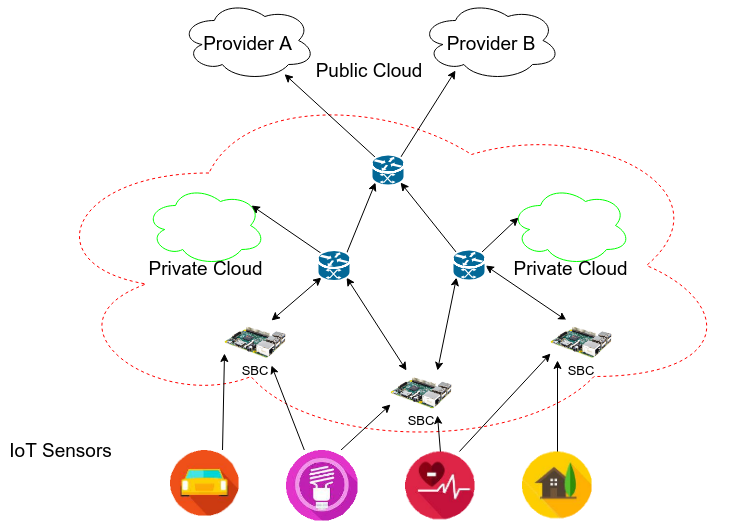
\includegraphics[width=0.5\linewidth]{figures/cassalesimgs-000.png}
%   \caption{\arch \cite{Cassales2019a} physical architecture and deployment scenario overview.}
%   \label{fig:mfog-phy-arch-cloud}
% \end{figure}

The overall \mfog architecture has two main modules, Classification and Novelty
Detection, which implement the \minas main tasks.
The Classification Module performs the same task of the \minas Online phase and
is the focal point for parallelism and distribution in our proposal.
It is replicated in the fog and runs on each cluster node, using a configurable
number of threads (limited to the node CPU core count).

The Novelty Detection Module can also be replicated,
the choice being one instance per local network, one global cloud instance,
or both.
This module also handles the homonymous task of \minas Online phase, receiving
all the samples labeled with \emph{unknown}, storing them in an internal
\emph{unknown-buffer}, and, when this buffer is full, performing the \minas
Novelty Detection task (clustering followed by validation).

\section{Polices}\label{sec:polices}

The design of our distributed \nd architecture includes partitioning the
functionalities of \minas and establishing the appropriate data flows
between different actors.
Changes to placement and behavior can have different impacts and should be
chosen with care.
The decisions following these discussions can be organized in several policies,
some of them were recurring during our implementation discussions and are:

\begin{itemize}
  \item Regarding the allocation of the Novelty Detection Module:
  \begin{itemize}
    
    \item At each fog node: patterns will be only detected if sufficient samples
    of them occur in the local observed network, use of the local node
    processing power, and a model synchronization mechanism between networks
    must be added;

    \item In the cloud: detect patterns even when scattered on each local
    network, each sample with \emph{unknown} label must be sent from edge to
    cloud implying increased internet link usage and increased delay between the
    appearance of a pattern, its detection and propagation to fog classifiers;

    \item On both: local \emph{unknown} buffer is maintained and novelty
    detection is local as well, once a sample is considered as noise or outlier
    it shall be sent to the cloud where the process repeats but with global
    data.
    This choice needs an even more complex model synchronization mechanism.

  \end{itemize}
    
  \item Regarding the model cleanup (forget mechanism): Even when a global
  novelty detection is used, local models can be optimized for faster
  classification using the local model statistics by sorting by (or removing)
  least used clusters;

  \item Lastly, reclassification of \emph{unknowns}: In the novelty detection
  task in \minas, the \emph{unknown} sample buffer is effectively classified
  using the new set of clusters.
  In Algorithm \ref{alg:MINAS-nd}, at the line \ref{alg:MINAS-nd:reclassify}, the
  new cluster valid (novelty or extension) includes the set of samples composing
  that cluster, thus, if this new label assignment was put forth to the system
  output it would introduce delayed outputs, more recent and perhaps more
  accurate.
  Also, it would change the system data stream behavior from a \emph{map}
  (meaning each input has one output) to a \emph{flatMap} (each input can have
  many outputs).

\end{itemize}


% Uma Implementação paralela do algoritmo de Detecção de Novidade em Streams MINAS

A Internet das Coisas (\iot) é composta por vastas quantidades de dispositivos
conectados à Internet e distribuídos geograficamente.
Com capacidades diversas providas por elementos como sensores e atuadores, esses
dispositivos produzem e consomem Fluxos Contínuos de Dados (\streams) com
diversos objetivos.
Alguns cenários de \iot envolvem a mineração desses fluxos (\streamMining) em busca de
padrões para tomada de decisão e, por vezes requerem também baixa latência.
Para casos de baixa latência ou alta vazão, conexões adequadas para
processamento em nuvem nem sempre são possíveis ou desejáveis; para esses casos,
a computação em névoa (\fog) é uma solução.

O tema de \streamMining envolve a classificação de novos elementos,
que podem tanto estar relacionados aos dados ou aos metadados das comunicações,
com base em um modelo.
\hlke{Porém, como \streams variam temporalmente e são ilimitados,}
as classes contidas em um \stream não são todas previamente conhecidas.
A identificação e classificação de novas classes em \streams é denominada
Detecção de Novidades (\novelty, \nd) em \streams.

\hlfa{Além dos aspectos}
\notafa{rever o parágrafo. Varios conceitos errados... a identificação de novas
classes é denominada detecção de novidade.... data stream variam temporalmente}
inerentes a \streamMining, são considerados na construção de um
\hlhl{sistema}
\notahl{Poderia reescrever a frase, evitando inversões na estrutura
sujeito/verbo e complementos. Yoda!}
que computa \streams a taxa de eventos
% (itens atômicos de um \stream)
gerados por cada produtor e o número de produtores nesse sistema, totalizando o
volume de eventos 
\notahl{qual sistema?}
\hlhl{do sistema}.
% Além do volume de eventos é necessário
Volumes elevados dificilmente são computados em apenas um nó (e muito menos em
um único núcleo processador) e por isso, esses sistemas \hlhl{geralmente} são distribuídos.

Sistemas que utilizam \nd para \streams gerados por dispositivos \iot devem
utilizar algoritmos que considerem os desafios inerentes a fluxos de dados
(\evolution e \drift) para adequada detecção de novidades e, para tanto,
requerem processamento em arquiteturas
que atendam os requisitos de volume de mensagens e latência de detecção.
O algoritmo MINAS é adequado para esse caso, pois trata os desafios de
\streamMining, porém não tem ainda implementação que atenda os requisitos de
volume e latência, especialmente para aplicações \iot onde um ambiente de \fog é
atrativo.

% \notahl{Com relação à proposta, será que é o caso de indicar que a
% arquitetura apresentada é uma proposta inicial, que será refinada ao longo da
% pesquisa?}

Para preencher a lacuna de algoritmo de \nd em ambiente \fog, propõem-se então
o \mfog, uma implementação do algoritmo MINAS sobre a plataforma \flink, que
considera distribuição em um ambiente de \fog.
O \mfog descrito neste documento foi refinado com os resultados dos experimentos
descritos na \refsec{resultados} e poderá ser revisado ao longo da pesquisa
conforme os resultados de outros experimentos evidenciarem obstáculos ou
oportunidades de melhoria.

% \nota{Reestruturar:
%   A - remember,
%   B - cenário (iot, fog, stream),
%   C - problema (4.1, ND em fog, terminar com minas e cassales),
%   D - solução (4.2, apresetnação, resumo \mfog, metodologia)
% }
% \nota{Falta: fog, processamento distribuído de streams, detecção de novidade}

\section{Descrição da Arquitetura Proposta}\label{sec:descricao}

\newcommand{\source}{módulo auxiliar \emph{source}\xspace}
\newcommand{\sink}{módulo auxiliar \emph{sink}\xspace}

\newcommand{\offline}{módulo treinamento\xspace}
\newcommand{\classify}{módulo classificador\xspace}
\newcommand{\detector}{módulo detector de novidades\xspace}

Nesta Seção, apresenta-se o \mfog, objeto proposta deste trabalho.
O \mfog é composto de três módulos principais e dois auxiliares.
Os módulos principais implementam o algoritmo MINAS, sendo eles: \offline
(\emph{Training Module}), \classify (\emph{Classification Module}) e
\detector (\emph{Novelty Detection Module}).
Dois módulos auxiliares são utilizados para avaliação do \mfog:
\source (fonte) e \sink (sorvedouro, consumidor final).
Os módulos e as interações entre eles são ilustradas na \reffig{arch}.

\begin{figure}[ht]
\centering
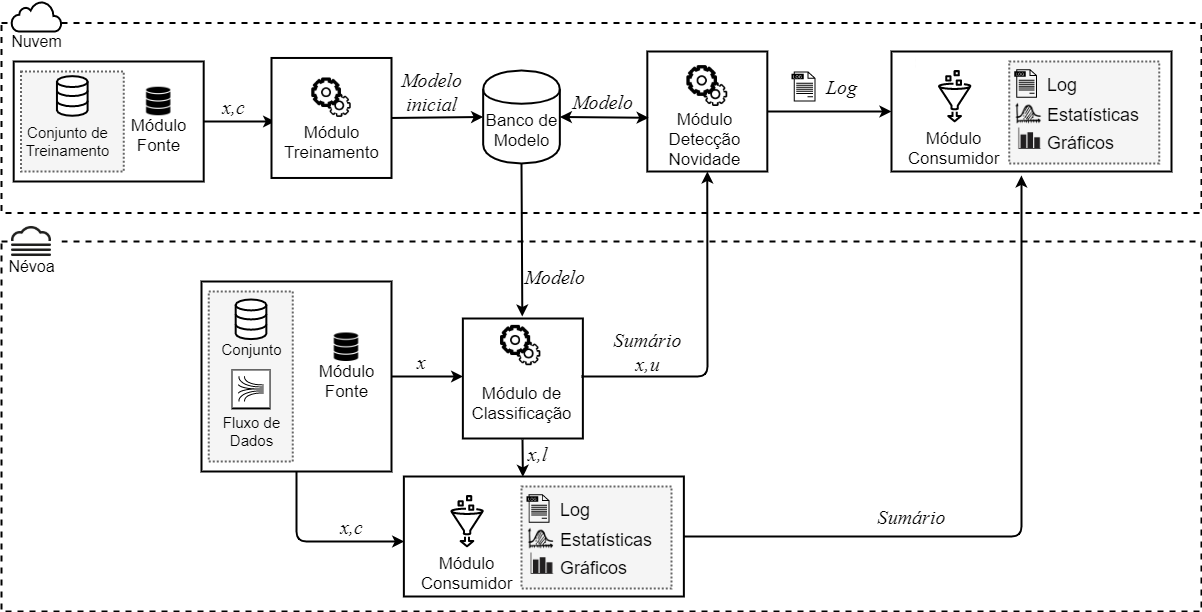
\includegraphics[width=\textwidth]{figuras/mfog-arch-v3_pt-br.png}
\caption{Arquitetura e fluxos de dados do \mfog.}
\label{fig:arch}
\end{figure}

A implementação do \mfog segue a arquitetura \arch formalizada por
\citeonline{Cassales2019a}, discutida na \refsec{cassales}.
A arquitetura \arch
% (e outras arquiteturas de NIDS)
estabelece que um serviço de
captura e tratamento de dados é instalado na borda de uma rede local com
dispositivos \iot.
Na presente implementação, esse serviço de captura e tratamento é representado
pelo \source.

O \source é dependente da fonte de dados, executando a transformação dos
formatos dos \datasets para um fluxo de exemplos (representado por $x$ na \reffig{arch})
compatível com o restante da implementação.
Além de fornecer exemplos tratados para o \classify, o \source também fornece
exemplos com a classe original (representado por $x,c$ na \reffig{arch})
\notafa{somente na fase de treinamento o source fornece exemplos rotulados par ao sink, certo?}
\hlfa{para o \sink e para o \offline}.

O \sink é responsável por agregar todos resultados do \mfog e,
juntamente com os valores do \dataset fornecidos pelo \source, por computar
as métricas de qualidade de classificação.
Além disso, esse módulo também coleta e agrega métricas base para as avaliação de
escalabilidade e métricas de uso de recursos computacionais.

Os dados resultantes do serviço de captura e tratamento (representado no \mfog
pelo \source) são ingeridos pela aplicação no \classify. A ingestão é feita por
meio de um operador fonte, fornecida pela plataforma \flink.
% \notake{TCP e apache flink}
% conexão TCP (\emph{Transmission Control Protocol}).
Na plataforma, com o modelo de classificação disponível, os exemplos são
classificados seguindo o algoritmo MINAS original discutido na \refsec{minas-og}.
A etiqueta atribuída pela classificação, ou meta-etiqueta de desconhecido,
juntamente com o exemplo original (representado por $x,l$ na \reffig{arch})
são enviados para o \sink.
Além disso, se o exemplo não for classificado, o exemplo e a meta-etiqueta de
desconhecido (representado por $x,u$ na \reffig{arch}) são enviados para o
\detector.
\notahl{processaa ND em paralelo?}
Outra comunicação é o envio das modificações ao sumário estatístico do modelo de
classificação (representado por $Summary$ na \reffig{arch}) do \classify para o
\detector.

O \detector é responsável por executar o processo de detecção de novidade,
atualizando o modelo de classificação, e entregar o novo modelo às instâncias do
\classify, através do serviço de armazenamento de modelo (\emph{Model Store} na
\reffig{arch}).
O \detector também envia meta-informações sobre o processo de detecção de
novidade (representado por $Log$ na \reffig{arch}) para o \sink.

% \nota{
% nao seria legal fazer um diagrama pq ai vc pode usar ate nos slides de como eh
% essa implementacao. Faz no draw io pra que de pra usar na monografia e de para
% enxergar na apresentacao
% }

O \mfog utiliza em seus módulos a distribuição oferecida pela plataforma \flink
como paralelização, ou seja, utiliza uma instância de trabalho (\emph{job}) por
dispositivo de classificação, sendo que cada instância de trabalho aloca um
gerenciador de tarefas por processador.
Dessa forma, busca-se a escalabilidade no ambiente de \fog para o \classify.
O \offline, por ser utilizado somente uma vez para gerar o modelo
de classificação inicial, não tem impacto na escalabilidade geral do sistema.
O \detector também é implementado na plataforma \flink e, por ser hospedado em
ambiente de \cloud, herda as qualidades desse ambiente incluindo escalabilidade.
\notake{destaque sentença}
O restante do sistema (\source, \sink, armazenamento de modelo) não é foco deste
estudo e sua escalabilidade, desde que não afete a escalabilidade do \classify e
\detector.
\notahl{Questões que precisam ser tratadas:\\
- Paralelização da classificação: como agrupar os dados e dividir o processamento?\\
- ND: como saber o que agrupar (dos nós) e como dividir?
Padrões podem ser locais? Ou sempre se aplicam a todos os nós?}
\notafa{frase incompleta}

% ------------------------------------------------------------------------------
\section{Metodologia de Avaliação}\label{sec:esperados}

% \nota{reestrutura 2:
%   A - cenario
%   B - metodologia (como, o que vai implementar [kafka, python, flink], como avaliar)
%   C - métricas (escalabilidade, qualidade)
%   D - resultados preliminares (python/kafka, flink)
% }

A avaliação da proposta apresentada é feita por meio de métricas extraídas da
literatura, divididas em duas partes: métricas de qualidade de classificação
e métricas de escalabilidade.
Métricas tradicionais de qualidade de classificação estabelecidas por trabalhos
de aprendizado de máquina não são adequadas para avaliar detecção de novidades em
\streams sem tratamento inicial. Felizmente, o tratamento necessário é
estabelecido por \citeonline{Faria2013} e expandido por
\citeonline{DaSilva2018,DaSilva2018thesis,Costa2019,Costa2019thesis}.
Além do tratamento estabelecido, as métricas tradicionais não são calculadas
somente para o conjunto completo, e sim para cada exemplo classificado.
Portanto, as métricas têm como índice o instante ($n$ nas equações à seguir),
informando a posição do exemplo em relação ao fluxo.

O tratamento estabelecido das métricas de qualidade para \streamMining define
que as métricas sejam extraídas de uma matriz de erro de classificação
multi-classe $\mathbf{E}_n$ (\refequ{matrix}), adaptada para detecção de
novidade.
A matriz de erro é preenchida com o número de eventos da classe $c_i$ classificados com
etiqueta $l_j$ até o instante $n$.
A \refequ{classes} representa o conjunto de classes presentes nos eventos
do fluxo até o instante $n$ e a \refequ{labels} representa o conjunto
de etiquetas atribuídas pelo classificador a eventos até o mesmo instante.

\begin{align}
  % x_n &= classify_{n-1}(x_n)\\
  % e_{i, j} &= classify_{n-1}(x_n)\\
  \mathbf{C}_n &= \{ c_1, c_2, \cdots, c_M \}  \label{eq:classes} \\
  \mathbf{L}_n &= \{ l_1, l_2, \cdots, l_J \}  \label{eq:labels} \\
  \mathbf{E}_n &= \begin{pmatrix}
    e_{1,1} & e_{1,2} & \cdots & e_{1,J} \\
    e_{2,1} & e_{2,2} & \cdots & e_{2,J} \\
    \vdots  & \vdots  & \ddots & \vdots  \\
    e_{M,1} & e_{M,2} & \cdots & e_{M,J} 
  \end{pmatrix}  \label{eq:matrix}
\end{align}

As métricas de qualidade de classificação selecionadas para avaliar a
implementação do \mfog serão
taxa de desconhecidos ($UnkR$ na \refequ{unkr}) \cite{Faria2013},
acurácia média ($acc$ na \refequ{acc})
e Macro F-score ($Fscore$ na \refequ{fscore}, também referido na literatura por
F1M) \cite{Sokolova2009,DaSilva2018thesis}.
As métricas são extraídas para todos os exemplos classificados (instantes $n$)
da respectiva matriz de erro $\mathbf{E}_n$.

% \nota{'para todos os instantes n' ??}

% \nota{Explicar o que significa cada elemento nas fórmulas}

\begin{align}
  \mathit{UnkR}_n       &= \frac{1}{M} \sum_{i=1}^{M} \frac{\#Unk_i}{\#ExC_i} \label{eq:unkr} \\
  \mathit{acc}_n        &= \frac{1}{M} \sum_{i=1}^{M} \frac{tp_i + tn_i}{tp_i+fn_i+fp_i+tn_i}
  = \frac{1}{M} \sum_{i=1}^{M} \frac{\#Acc_i}{\#ExC_i}  \label{eq:acc} \\
  \mathit{Precision}_n  &= \frac{1}{M} \sum_{i=1}^{M} \frac{tp_i}{tp_i+fp_i} \\
  \mathit{Recall}_n     &= \frac{1}{M} \sum_{i=1}^{M} \frac{tp_i}{tp_i+fn_i} \\
  \mathit{Fscore}\beta_n &= (\beta^2 +1) \cdot
  \frac{
  \mathit{Precision} \cdot \mathit{Recall}
  }{
    \beta^2 \cdot \mathit{Precision} +\mathit{Recall}
  }\\
  \mathit{Fscore}1_n   &= 2 \cdot \frac{
    \mathit{Precision} \cdot \mathit{Recall}
    }{
      \mathit{Precision} +\mathit{Recall}
    } \label{eq:fscore}
\end{align}
% = 2 \cdot \frac{tp}{2 \cdot tp + fn + fp}
% \mathcal{L}         &= \frac{-1}{N} \sum_{i=1}^{M} \sum_{j=1}^{J} y_{i,j} \log(p_{i,j})

% \nota{usar coeficiente d-intra vs d-extra grupo para determinar K de
% cada label. Também pode-se usar os mesmos coeficientes para _log_}

A transformação do fluxo de saída em uma matriz de erro é realizada no \sink,
\notahl{como tratar o paralelismo desse elemento?\\
Ele dá conta de todo o fluxo recebido dos classificadores?}
\hlhl{onde} 
\hlhl{tem-se disponível o fluxo original}
\hlhl{com as etiquetas corretas e o fluxo resultante}
\hlhl{da classificação.}
Esse módulo deve levar em consideração que pode haver reclassificação de um
evento, previamente rotulado como desconhecido, em padrões oriundos de classe
novidade ou extensão devido ao processo de detecção de novidades executado
posteriormente ao surgimento do padrão em questão.

% Portanto os resultados são computados em função do fluxo de saída, então os $n$ nas
% equações são o índice do evento de saída.
% $\mathbf{unk}$ é o conjunto de eventos marcados como desconhecidos.
% \nota{oque eh unk? nesse paragrafo acima, erro de compilacao do latex?}

% \nota{frase confusa, eh so tirar o COMO e quebrar a frase: Esse módulo deve levar em consideração que
% COMO pode haver reclassificação de um evento, previamente rotulado como
% desconhecido, em padrões oriundos de classe novidade ou extensão devido ao
% processo de detecção de novidades executado posteriormente ao surgimento
% do padrão em questão}

% \begin{align}
%   E_{n,i,j} &= \bordermatrix{~ & c_i & \neg c_i \cr
%   l_j       & TP = \alpha           & FP = \gamma - \alpha                 \cr
%   \neg l_j  & FN = \beta - \alpha   & TN = n - (\alpha + \beta + \gamma)  \cr} \\
%   FM1       &= \frac{TP}{TP+\frac{FP+FN}{2}}
% \end{align}

% Os valores da matriz de erro para 

% \begin{align}
%   \alpha _j &= max( \{ |e_{i,j}|: i = 1 .. I \wedge \in \mathbf{E}_n \})
%           & \text{máximo da linha (etiqueta)} \\
%   a_j &= i: |e_{i,j}| = \alpha _j
%           & \text{índice da classe associada à etiqueta} \\
%   \beta   &= \sum_{j = 0}^{J} e_{i,j} : e_{i,j} \in \mathbf{E}_n
%           & \text{soma de uma coluna (etiqueta)} \\
%   \gamma  &= \sum_{i = 0}^{I} a_{i,j} : e_{i,j} \in \mathbf{E}_n
%           & \text{soma de uma linha (classe)}
% \end{align}

As métricas de escalabilidade selecionadas são: número de nós processadores,
tipo de processadores, uso de memória, tempo de processamento, taxa de eventos
processados e latência entre a produção e classificação de um evento.

% \begin{align}
%   \Delta { } t_n       &= t_{n,sink} - t_{n,source} \label{eq:delta-t} \\
%   \overline{\Delta { } t}_n       &= \frac{1}{N} \sum_{i=1}^{N} \Delta { } t_n  \label{eq:avg-delta-t} \\
%   \alpha &= \# processors \\
%   \gamma &= \frac{\overline{\Delta { } t}}{}
% \end{align}

% \nota{
% como assim os resultados sao validos so se tiverem essas metricas? Entao quer
% dizer que qual medida eh valida? Vc quis dizer que se as medicoes que vc extrair
% com essas metricas forem iguais as medicoes do minas original, entao ai eh
% valido. Eh Isso?
% }

Da implementação do \mfog é prevista a execução de experimentos com \datasets
diversos, em especial os \datasets reais como \emph{Kyoto 2006+},
que contenham evolução de conceitos.
Os resultados desses experimentos irão conter as seguintes métricas:

\begin{enumerate}[label={\alph*)}]
  \item Qualidade de classificação (taxa de desconhecidos, F1M);
  \item Escalabilidade (número de processadores, volume processado, tempo
  decorrido);
  \item Recursos computacionais utilizados (memória, tempo de processamento,
  operações de leitura e escrita).
\end{enumerate}

Para a validação da corretude da implementação do \mfog com relação ao algoritmo
MINAS original, as métricas de qualidade de classificação serão extraídas de
ambas as Implementação e comparadas.
